\documentclass[unicode, dvipsnames]{beamer}

\usetheme{Madrid} %тема
\usecolortheme{whale} %цветовая гамма
%Выбирать тему и цветовую гамму презентации очень удобно на http://www.hartwork.org/beamer-theme-matrix/

\usefonttheme[onlylarge]{structurebold} % названия и текст в колонтитулах выводится полужирным шрифтом.
\usefonttheme[onlymath]{serif}  % привычный шрифт для математических формул
\setbeamerfont*{frametitle}{size=\normalsize,series=\bfseries} % шрифт заголовков слайдов

%Русификация
\usepackage[utf8]{inputenc}
\usepackage[russian]{babel}

%Для вставки рисунков
\usepackage{graphics, graphicx}
\usepackage{epstopdf}
\usepackage[normalem]{ulem}
\usepackage{transparent}

\usepackage[nopar]{lipsum} %для генерации большого текста

%Для вывода листинга TeXовского кода
\usepackage{listings}
\usepackage{color}
\usepackage{textcomp}
\usepackage{dsfont}
\usepackage{tabularx}
\usepackage{bm}

\DeclareMathOperator*{\argmin}{arg\,min}

\usepackage{array}
\newcolumntype{L}[1]{>{\raggedright\let\newline\\\arraybackslash\hspace{0pt}}m{#1}}
\newcolumntype{C}[1]{>{\centering\let\newline\\\arraybackslash\hspace{0pt}}m{#1}}
\newcolumntype{R}[1]{>{\raggedleft\let\newline\\\arraybackslash\hspace{0pt}}m{#1}}

\title[Time Series Alignment]{Differentiable Dynamic Programming \\ for Time Series Alignment}
\author[]{Тимур Гарипов, 517 группа \\ Татьяна Шолохова, 517 группа \\ Павел Коваленко, 517 группа \\ Саня Щербаков, 522 группа}

\date{9 июня 2018}

\begin{document}

%Титульный слайд
\begin{frame}
    \titlepage
\end{frame}

\begin{frame}{Постановка задачи}
	Рассматривается задача выравнивания временных рядов.
	
	\bigskip
	Дана нотная запись музыкальной композиции и аудиозапись этой композиции. Требуется каждому моменту времени в аудиозаписи сопоставить ноту, играемую в этот момент.
	
	\bigskip
	\centering
	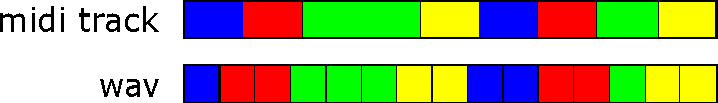
\includegraphics[width=0.8\textwidth]{graphics/task.pdf}
\end{frame}

\begin{frame}{Описание датасета}
В работе был использован датасет \href{http://music.cs.northwestern.edu/data/Bach10.html}{Bach 10}, состоящий из 10 аудиозаписей фрагментов хоралов Баха, продолжительность фрагментов --- от 25 до 40 секунд. 

\bigskip
Каждая запись состоит из четырех дорожек, соответствующих четырем инструментам --- скрипка, кларнет, саксофон и фагот. Есть как записи отдельных дорожек, так и сводная запись всех инструментов.

\bigskip
Для каждой дорожки дана ее идеальная нотная запись, однако фактическая игра от нее немного отклоняется. Также для всех дорожек дано правильное выравнивание аудио-- и нотной записи. Для инструментов в выборке представлено от 15 до 25 различных нот.

\end{frame}

\begin{frame}{Выравнивание}

Для аудиозаписи выделим с равными интервалами ключевые точки, для которых будем искать выравнивание. 

Выравнивание можно представить в виде бинарной матрицы $Y$ размера количество нот $\times$ количество фрагментов в разбиении. Единица в позиции $(i, j)$ означает, что в $j$--й момент времени проигрывалась $i$--я нота.

\bigskip
\centering
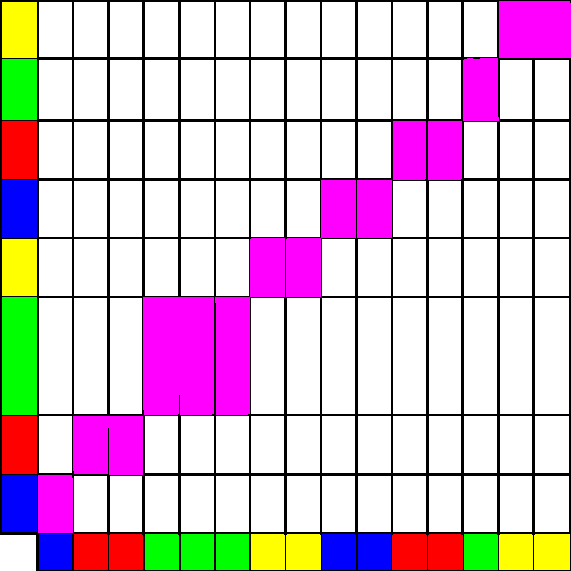
\includegraphics[width=0.35\textwidth]{graphics/task2.pdf}
\end{frame}

\begin{frame}{Выравнивание}

Предположим, что последовательность нот при игре не изменилась и ни одна из нот не была пропущена. Тогда выравнивание можно представить в виде пути в матрице $Y$ из левой верхней клетки правую-нижнюю, при этом разрешены перемещения только вправо, вниз и вправо-вниз. Пример выравнивания --- на рисунке ниже.

\bigskip
\centering
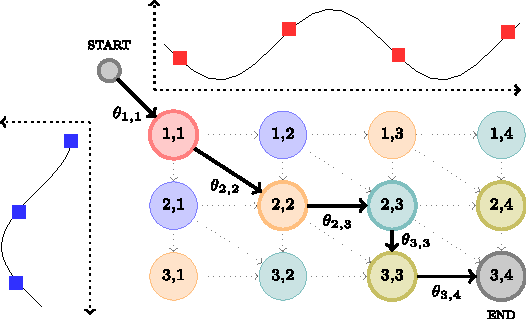
\includegraphics[width=0.6\textwidth]{graphics/align_example.pdf}

\end{frame}

\begin{frame}{Метрика качества}

Выбирая мелкие интервалы разбиения аудиозаписи, можно добиться, чтобы в каждый момент времени играла только одна нота. Тогда целью задачи является предсказать каждого момента разбиения какая нота играет. 

\bigskip
Для матрицы это ограничение означает, что в каждом столбце может быть не больше одной единицы. Для пути в графе это ограничение равносильно запрету переходов вниз.

\bigskip
Метрика качества --- \textit{mean absolute deviation} --- суммарное (по моментам времени) отклонение индекса предсказанной ноты от истинного индекса.

\end{frame}

\begin{frame}{Аудио признаки}

В статье предложено использовать следующие признаки для аудиодорожки:

\bigskip
\begin{itemize}
	\item MFCC признаки --- первые 5 коэффициентов.
	\item Root Mean Square Energy --- энергия фрейма.
	\item Spectral Centroid --- средняя частота спектра во фрейме.
	\item Spectral Bandwidth --- разброс частот спектра во фрейме.
\end{itemize}

\bigskip
Были использованы реализации этих признаков из библиотеки librosa.

\end{frame}

\begin{frame}{Простое решение}
	Разбиваем датасет на две части.
	На первой части обучаем классификатор по числу различных нот --- предсказываем вероятность того, что в момент времени $t$ играет нота~$i$.
	
	\bigskip
	Для второй части датасета построим матрицу $\theta \in \mathds{R}^{N_A \times N_B}$. 
	
	$\theta_{ij}$ соответствует отрицательному логарифму вероятности того, что в момент времени $j$ играет нота номер $i$, то есть штрафу за предсказание ноты $i$ для момента времени $j$. Этот штраф можно получить из классификатора.
	
	\bigskip
	Теперь требуется найти в матрице путь из клетки $(1, 1)$ в клетку $(N_A, N_B)$ с наименьшим суммарным штрафом. Эту задачу можно решить за $N_A \times N_B$ операций при помощи динамического программирования.
	
\end{frame}

\begin{frame}{Поиск минимального пути}

Дана матрица $N_A \times N_B$ штрафов. Нужно найти путь из клетки $(1, 1)$ в клетку $(N_A, N_B)$ с наименьшим суммарным штрафом. На пути из клетки можно перемещаться в ее соседа справа или справа-снизу.

\bigskip
Заведем матрицу $D$ размера $N_A \times N_B$. $D_{ij}$ равно минимальному штрафу, за который можно проложить путь из $(1, 1)$ в $(i, j)$. Будем заполнять эту матрицу по столбцам.

\bigskip
\textbf{База динамики}

$D_{11} = \theta_{11}$, $D_{1j} = +\infty$

\bigskip
\textbf{Шаг динамики}

$D_{ij} = \min(D_{i-1, j}, D_{i-1, j-1}) + \theta_{ij}$

\end{frame}

\begin{frame}{Differentiable Dynamic Programming}{Smoothed max/min operators}
Рассмотрим $x \in \mathbb{R}^d$
\[
	\min(\bm{x}) = \min\limits_{i=1,\ldots,d} x_i
\]	

Пусть $\Omega(\cdot): \mathbb{R}^d \to \mathbb{R}$ ~--- cильно выпуклая функция
\[
	\min{}_{\Omega}(\bm{x}) = \min\limits_{\bm{q} \in \Delta^d} \langle \bm{q}, \bm{x}\rangle + \Omega(\bm{q}).
\]

Тогда $\min{}_{\Omega}(\bm{x}$)~--- гладкая функция:

\[
	\nabla_{\bm{x}} \min{}_{\Omega}(\bm{x}) = \argmin\limits_{\bm{q} \in \Delta^d} \langle \bm{q}, \bm{x}\rangle + \Omega(\bm{q})
\]
\end{frame}

\begin{frame}{Differentiable Dynamic Programming}{Пример}

Например:
\[
	\Omega(\bm{q}) = \gamma \sum_{i=1}^d q_i \log q_i, \quad \gamma > 0
\]

\[
\min{}_{\Omega}(\bm{x}) = \min\limits_{\bm{q} \in \Delta^d} \sum_{i=1}^d q_i x_i + \gamma \sum_{i=1}^d q_i \log q_i 
\]

\[
	\hat q_i \propto \exp\left\{-\frac{x_i}{\gamma}\right\}, \quad \hat{\bm{q}} = \mathrm{softmax}\left(-\frac{\bm{x}}{\gamma}\right)= \mathrm{softmin}\left(\frac{\bm{x}}{\gamma}\right)
\]
	
\end{frame}

\begin{frame}{Differentiable Dynamic Programming}{Выравнивание}
	
Пусть $\theta \in \mathbb{R}^{N_A \times N_B}$. 

\begin{itemize}
	\item Алгоритм $\mathrm{DTW}$:
	\begin{itemize}
		\item $\mathrm{DTW}(\theta)$~--- величина минимального пути;
		\item $Y(\theta) \in \{0, 1\}^{N_A \times N_B}$~--- матрица выранивания;
	\end{itemize}
	\item Алгоритм  $\mathrm{DTW}_\Omega$:
	\begin{itemize}
		\item $\mathrm{DTW}_\Omega(\theta)$~--- приближенная величина минимального пути;
		\item $Y_\Omega(\theta) = \nabla_\theta \mathrm{DTW}_\Omega(\theta)$~--- сглаженная матрица выранивания;
	\end{itemize}
\end{itemize}	
	Оптимизируемый функционал:
	\[
	\mathrm{MAD}(\hat Y, Y) = \|L(Y - \hat Y)^T\|^2_F,
	\]
	где $L \in \mathbb{R}^{N_B \times N_B}$~--- нижнетреугольная матрица, заполненная $1$.
\end{frame}

\begin{frame}{Differentiable Dynamic Programming}{Алгоритм}
	\begin{figure}		
		\centering
		\vspace{-0.2em}
		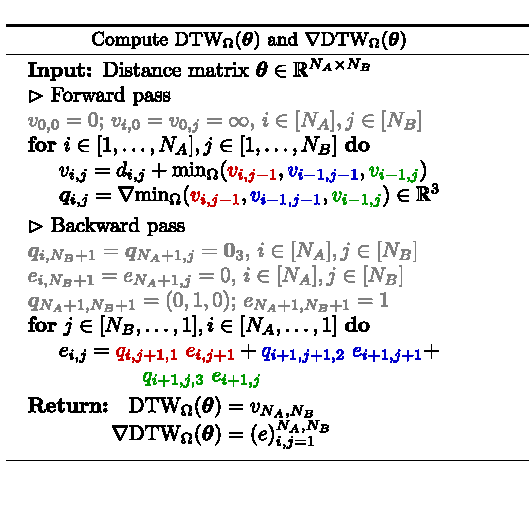
\includegraphics[height=0.85\textheight]{./graphics/alg.pdf}
	\end{figure}
\end{frame}


\begin{frame}{Результаты экспериментов}

Выборка была разбита на тренировочную и валидационную, по пять записей в каждой из частей.

\bigskip
Были рассмотрены три модели: 
\begin{enumerate}
	\item Простая модель с логистической регрессией в качестве базового классификатора.
	\item End-to-end модель на основе $\mathrm{DTW}_\Omega$.
\end{enumerate}

\bigskip
\centering
\begin{tabular}{|l|c|c|}
	\hline
	Инструмент & Pretrained & End-to-end \\
	\hline
	Скрипка & 0.7804 & 0.4761 \\
	\hline
	Кларнет & 0.4527 & 0.2353 \\
	\hline
	Саксофон & 0.4930 & 0.4677 \\
	\hline
	Фагот & 0.6001 & 0.5650 \\
	\hline
\end{tabular}

\end{frame}

\begin{frame}{Вклад участников}

{\bfseries Тимур Гарипов}\\ 

Реализация метода End-to-end на основе алгоритма $DTW_{\Omega}$.\\
\bigskip
{\bfseries Татьяна Шолохова}\\ 

Подготовка данных и извлечение признаков для классификатора.\\
\bigskip
{\bfseries Павел Коваленко}\\

Реализация простой модели с логистической регрессией в качестве базового классификатора.\\
\bigskip
{\bfseries Саня Щербаков} \\

Проведение экспериментов. Рефакторинг и документация кода. 

\end{frame}

\begin{frame}{}

\centering

\includegraphics[width=0.6\textwidth]{graphics/final.jpg}

\bigskip
\textbf{Состав команды:}

Тимур Гарипов, 517 группа \\ Татьяна Шолохова, 517 группа \\ Павел Коваленко, 517 группа \\ Саня Щербаков, 522 группа

\end{frame}

\end{document}